\section {Environmental disturbance torques}
  \label{chap:distTorques}
%
Disturbance torques can be classified either as external or internal \todo{don't distinguish between external and internal}. Since the external disturbances are larger in magnitude compared to \todo{reference} internal and can cause a change in the total momentum of the spacecraft, only these will be accounted. The external disturbing torques that will be discussed are aerodynamic, solar radiation and gravity gradient torque.
\subsection*{Aerodynamic disturbance torque}\label{chap:disturbances}
%
Gas molecules, in a LEO(low Earth orbit) collide with the surface of the satellite causing
a force which direction opposes the direction of the satellites velocity vector. This Aerodynamic force can be modelled as \cite{SADC,our_report}  


\begin{flalign}
	\vec{F_A} = -\frac{1}{2} \rho \ C_D \ A_{\perp}   \vec{v}^2
	\label{eq:ec1c}
\end{flalign}

where $\rho$ is the atmospheric density  
is chosen to be constant and equal to $1.454 \cdot 10^{-13} Kg/{m^3}$ based on the Committee on Space Research\cite{FSA}, $\vec{v}$ is the satellite velocity vector, $A_{\perp}$ is the area perpendicular to the velocity and $C_D$ is the drag coefficient and is usually chosen to be equal to 2 \cite{SADC}\cite{our_report}  . If the calculation of the lifetime of the satellite is of great importance a more accurate drag coefficient should be used.

\begin{figure}[h!]
	\centering
	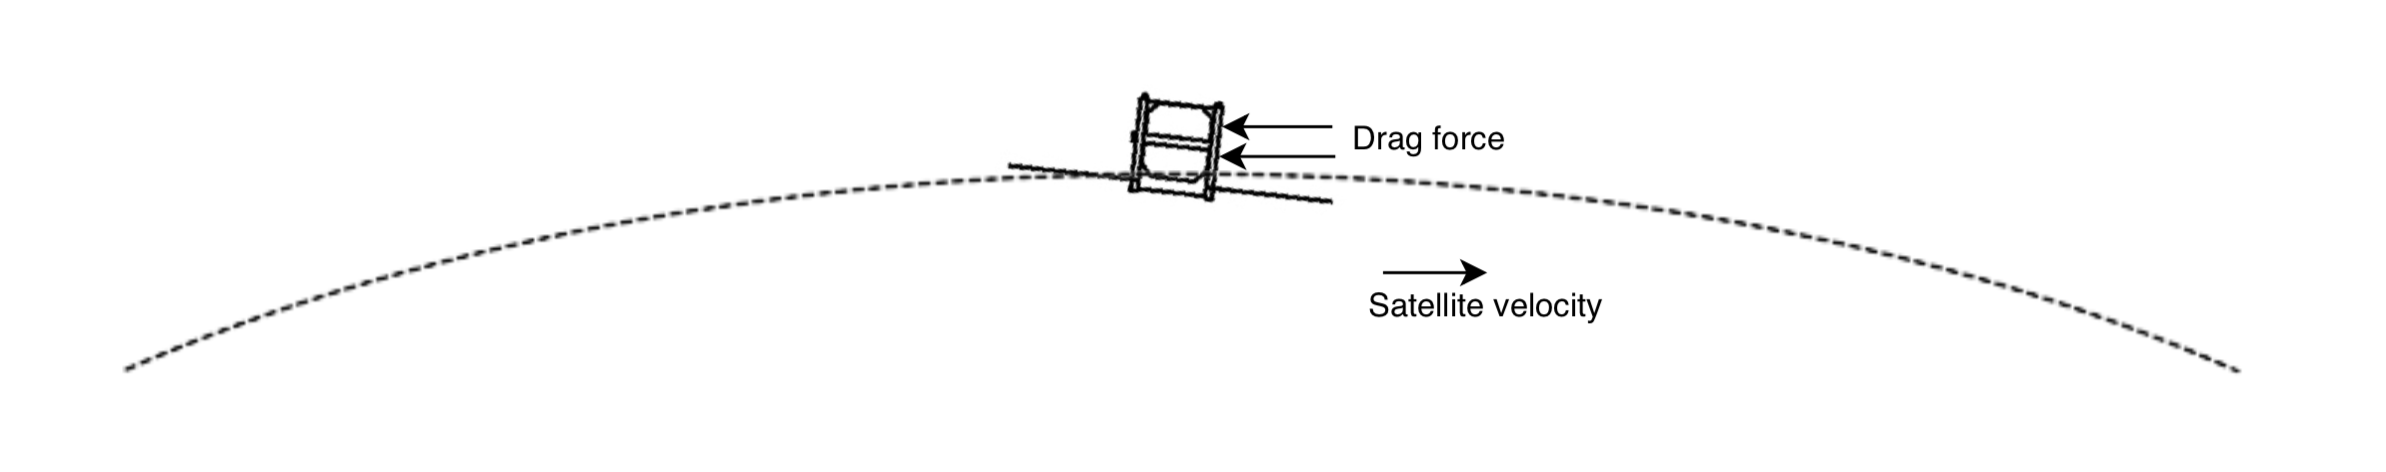
\includegraphics[width=0.9\linewidth]{figures/AFF}
	\caption{Aerodynamic disturbance force actiong on the satellite on orbit}
	\label{fig:af}
\end{figure}

Using the \eqref{eq:ec1c}, the aerodynamic torque acting on the satellite can be written as 
\begin{flalign}
	\vec N_{drag} = \vec r_{s} \times  \vec F_{A} 
	\label{eq:drag}
\end{flalign}
where:\\
$\vec r_{s}$ is the vector from the centre of mass of the satellite to the geometric centre of the exposed area

\subsection*{Solar radiation disturbance torque}\label{chap: disturbances2}

Solar radiation pressure is emitted from various sources such as reflection from the Earth's atmosphere, from solar wind and direct radiation from the sun to the surface of the satellite\cite{SADC}\cite{our_report}  . Direct radiation is larger and only this source will be taken into account.

\begin{table}[H]
	\begin{minipage}[b]{0.49\linewidth}
		\centering
		\begin{figure}[H]
			\centering
			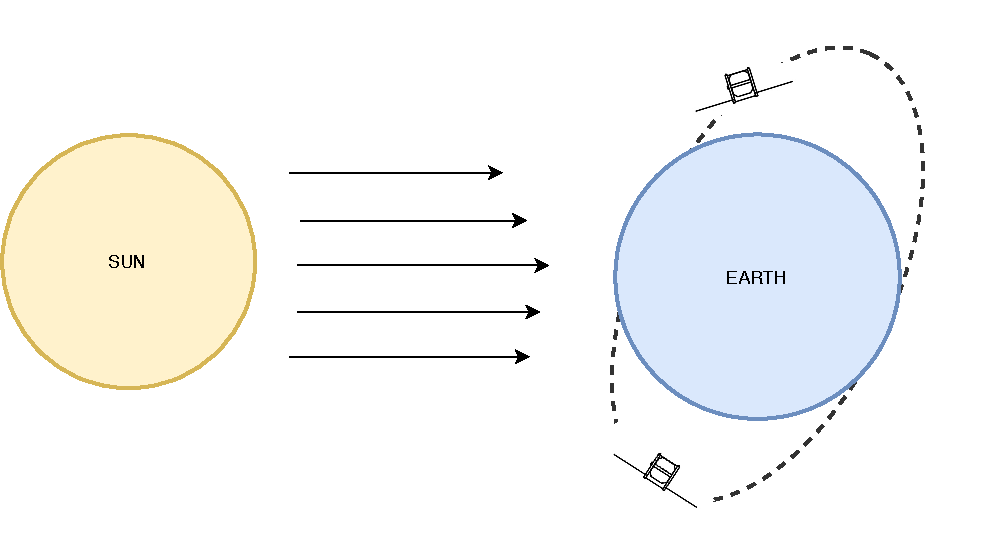
\includegraphics[width=1\linewidth]{figures/sunRAD}
		
		\end{figure}
	\end{minipage}\hfill
	\begin{minipage}[b]{0.49\linewidth}
		\centering
		\begin{figure}[H]
			\centering
			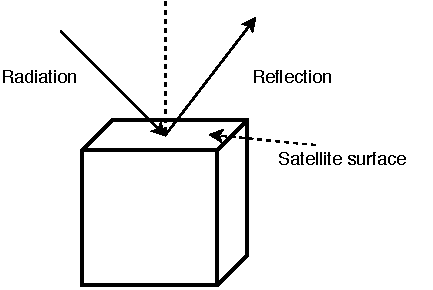
\includegraphics[width=0.55\linewidth]{figures/solarRad}
		
		\end{figure}
	\end{minipage}
	\caption{ Sun radiation actiong on satellite surface}
	\label{fig:radf}
\end{table}

The solar flux is given as
\begin{flalign}
	P = \dfrac{F_s}{c}
	\label{eq:flux2}
\end{flalign}

where $F_s$ is the intensity or mean energy flux given as 1358 [$W/m^2$] and $c$ is the speed of light. The solar radiation force $\vec F_{rad}$ can be expressed as 

\begin{flalign}
	\vec {F_{rad}} = C_{a} P A \ \hat{S}
	\label{eq:Pres}
\end{flalign}
where $C_{a}\in [0,2]$ is the absorption coefficient which depends on the material of the satellite with 2 \todo{decide if 1.5 or 2 should be used} be the value of totally reflected beam, $P$ is the solar flux, $A$ is the radiated surface area, and $\hat{S} =\frac{\vec {r_{sun,sat}}}{||\vec {r_{sun,sat}}||}$ is the unit vector from the satellite to the sun. The solar radiation torque can be computed as 
\begin{flalign}
	\vec N_{solar} = \vec r_{s} \times  \vec F_{rad} 
	\label{eq:solar}
\end{flalign}
where $\vec r_{s}$ is the vector from the center of mass of the satellite to the center of pressure.
%
\subsection*{Gravity Gradient disturbance torque and $J_2$  perturbation}\label{chap: disturbances3} \todo{separate}
%
Due to the non spherical mass distribution and non homogeneity of the Earth, a pertubative gravitational force($J_{2}$ perturbation)\cite{SADC}\cite{our_report} exerted on the satellite determining its orbit difference compared to ideal mathematical models.
Contrary to this, in order to derive an expression for the gravitational torque exerted about the mass centre of the satellite, it will be assumed symmetrical, spherical distribution of the Earth's mass\cite{SADC} with this assumption be valid by comparing the magnitude of the gravity gradient with the other pertubative torques.     
\subsubsection{$J_2$ gravity perturbation}
An approximation of the gravitational potential of the Earth is \cite{SADC}\cite{our_report}:
\begin{flalign}
	U \approx -\frac{\mu}{r} \left[1 - \sum_{n=2}^{\infty} \left(\frac{R_e}{r}\right)^{n} J_n P_n sin(\phi)  \right ] = \frac{\mu}{r} [U_0 + U_{J_2} + U_{J_3} + ...]
	\label{eq:Pr341}
\end{flalign}
which has been derived using the spherical harmonic expansion describing deviations of the potential to the south and north direction,
with $U_0$ = -1, $U_{J_2}$ = $\left(\frac{R_e}{r}\right)^{2} J_2 \frac{1}{2} (3 sin^2 \phi -1) $ and ${J_2}$ be a numerical coefficient, with the other terms been discarded.

The final relation is obtained as 
\begin{flalign}
	\vec F = -m \nabla U
	\label{eq:Pr3431}
\end{flalign}
with the vector $\vec F$ expand to the components \cite{SIDI}\cite{our_report}  :
\begin{flalign}
	F_x = -\frac{\partial U}{\partial x} = \mu \left[ -\frac{x}{r^3} + A_{J_2} \left(15 \frac{xz^2}{r^7} - 3\frac{x}{r^5}   \right ) \right ]       \\
	F_y = -\frac{\partial U}{\partial y} = \mu \left[ -\frac{y}{r^3} + A_{J_2} \left(15 \frac{yz^2}{r^7} - 3\frac{y}{r^5}   \right ) \right ]       \\
	F_z = - \frac{\partial U}{\partial z} =  \mu \left[ -\frac{z}{r^3} + A_{J_2} \left(15 \frac{z^3}{r^7} - 3\frac{z}{r^5}   \right )  \right]       
	\label{eq:Pr34331}
\end{flalign}
where $A_{J_2}  = \frac{1}{2} J_2 R_e^2$ and and $R_e$ is the mean radius o the Earth at the equator
%
%
\subsubsection{Gravity-Gradient torque}
The gravity gradient effect about the centre of mass of the satellite is a consequence of the non uniform gravitational field of the Earth. The torque about the centre of mass of the satellite can be expressed as\cite{SADC}\cite{our_report}  

\nomenclature[A]{\textbf{COM}}{Center of Mass}
%
\begin{flalign}
	\vec N_{gg} &= \dfrac{3\mu}{\vec R_{sc}^3}[\vec{\hat R_{sc}} \times(\vec{I} \ \vec{\hat R_{sc}}] 
	\label{eq:ref4}
\end{flalign}
where $\vec{\hat R_{sc}}$ is the unit vector from geometric centre of the earth's to the satellite's geometric centre, $\mu = G*m_{earth}$ with $G$ be the Gravitational constant $6.6740*10^{-11}$ [$m^{3} kg^{-1} s^{-2}$] and $\underline I$ is the inertia matrix of the satellite. 

\begin{figure}[H]
	\centering
	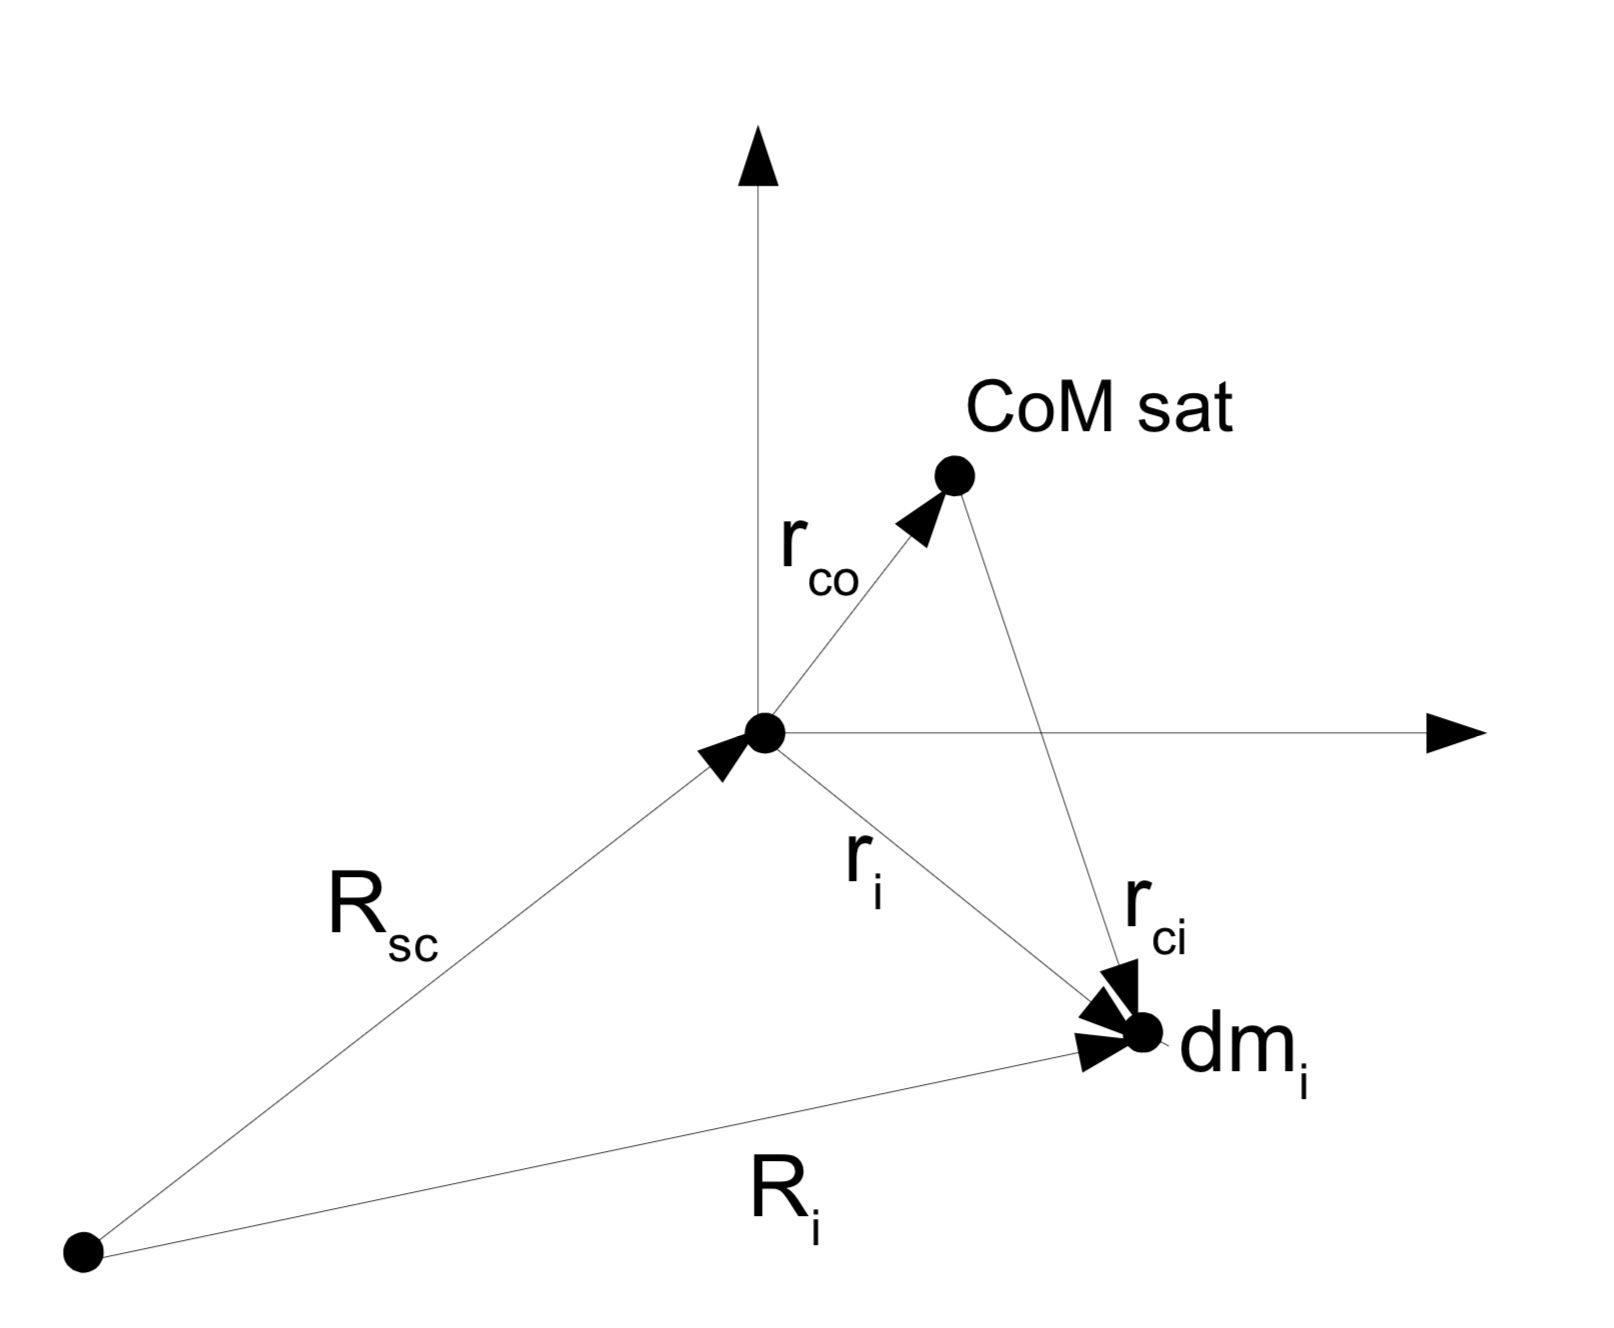
\includegraphics[width=0.5\linewidth]{figures/ggt}
	\caption{Gravity gradient torque computation using the coordinate system}
	\label{fig:gg}
\end{figure}

\subsection{Magnetic residual }
When the satellite orbits the Earth, due to the interference of the magnetic field of the Earth and the satellite magnetic residual, an extra disturbance torque is generated. Because the satellite can not be perfectly isolated, the actuators and sensors will produce a residual magnetic moment. Similarly like magnetorqers, the torque generated by the magnetic residual can be computed using:
\begin{flalign}
\vec N_{mr} = \vec m \times \vec B
\label{eq:st}
\end{flalign}
where $\vec m$ is the magnetic moment and $\vec B$ is the magnetic field of the Earth.

The magnetic field of the Earth can be approximated using \cite{SMAD}:
\begin{flalign}
B = \dfrac{2M}{R^3}
\label{eq:ftf}
\end{flalign}
where $M$ is the Earth magnetic moment and $R$ is the distance from the Earth to the center of the satellite.

\nomenclature[SNmr]{$\vec N_{mr}$}{The torque generated by the magnetic residual }
\nomenclature[Smr]{$\vec m_{mr}$}{The magnetic residual}
\nomenclature[SB]{$\vec B$}{The magnetic field of the Earth}
\nomenclature[SM]{$\vec M$}{The Earth magnetic moment }
\nomenclature[SR]{$\vec R$}{The distance from the Earth to the center of the satellite}
\subsection{Total disturbance torque}
The total disturbance torque acting on the satellite in the SBRF is:

\begin{flalign}
	N_{dist} = N_{drag} + N_{solar} + N_{gg} + N_{mr}
	\label{eq:TDT}
\end{flalign}